\documentclass[tikz]{standalone}
\usepackage{pgfplots}
\pgfplotsset{compat=1.15}
\usepackage{mathrsfs}
\usetikzlibrary{arrows,calc}
\usepackage{tkz-euclide}

\pagestyle{empty}

\definecolor{AngleClr}{rgb}{0,0.39215686274509803,0}
\definecolor{ShapeClr}{rgb}{0.6,0.2,0}
\definecolor{BlueClr}{RGB}{5,81,163}

\begin{document}

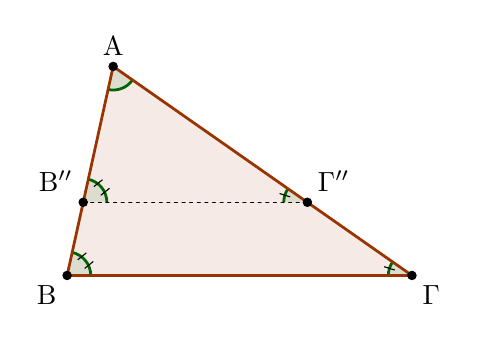
\begin{tikzpicture}[scale=.75]
\tkzSetUpLine[line width=1pt,color=black]
\tkzSetUpPoint[fill=black]

\tkzDefPoints{-3.5/0.84/A,-4.28/-2.7/B,1.56/-2.7/C}
\tkzDefPointOnLine[pos=0.65](A,B)\tkzGetPoint{BB}
\tkzDefPointOnLine[pos=0.65](A,C)\tkzGetPoint{CC}

\tkzFillPolygon[fill=ShapeClr,fill opacity=0.1](A,B,C)

\tkzFillAngle[fill=AngleClr,size=.4,fill opacity=0.1](B,A,C)
\tkzMarkAngle[line width=1pt,color=AngleClr,size=.4](B,A,C)

\tkzFillAngles[fill=AngleClr,size=.4,fill opacity=0.1](C,B,A CC,BB,A)
\tkzMarkAngles[mark=||,mksize=2,line width=1pt,color=AngleClr,size=.4](C,B,A CC,BB,A)

\tkzFillAngles[fill=AngleClr,size=.4,fill opacity=0.1](A,C,B A,CC,BB)
\tkzMarkAngles[mark=|,mksize=2,line width=1pt,color=AngleClr,size=.4](A,C,B A,CC,BB)

\tkzDrawSegments[line width=0.5pt,color=black,dashed,dash pattern=on 1pt off 1.75pt](BB,CC)


\tkzDrawPolygon[color=ShapeClr](A,B,C)

\tkzDrawPoints[size=3](A,B,C,BB,CC)

\tkzLabelPoint[above](A){$\rm A$}
\tkzLabelPoint[below left](B){$\rm B$}
\tkzLabelPoint[below right](C){$\rm \Gamma$}
\tkzLabelPoint[above left](BB){$\rm B''$}
\tkzLabelPoint[above right](CC){$\rm \Gamma''$}


\end{tikzpicture}

\end{document}
